\documentclass[ignorenonframetext,]{beamer}
\setbeamertemplate{caption}[numbered]
\setbeamertemplate{caption label separator}{: }
\setbeamercolor{caption name}{fg=normal text.fg}
\beamertemplatenavigationsymbolsempty
\usepackage{lmodern}
\usepackage{amssymb,amsmath}
\usepackage{ifxetex,ifluatex}
\usepackage{fixltx2e} % provides \textsubscript
\ifnum 0\ifxetex 1\fi\ifluatex 1\fi=0 % if pdftex
  \usepackage[T1]{fontenc}
  \usepackage[utf8]{inputenc}
\else % if luatex or xelatex
  \ifxetex
    \usepackage{mathspec}
  \else
    \usepackage{fontspec}
  \fi
  \defaultfontfeatures{Ligatures=TeX,Scale=MatchLowercase}
\fi
\usefonttheme{structurebold}
% use upquote if available, for straight quotes in verbatim environments
\IfFileExists{upquote.sty}{\usepackage{upquote}}{}
% use microtype if available
\IfFileExists{microtype.sty}{%
\usepackage{microtype}
\UseMicrotypeSet[protrusion]{basicmath} % disable protrusion for tt fonts
}{}
\newif\ifbibliography
\usepackage{longtable,booktabs}
\usepackage{caption}
% These lines are needed to make table captions work with longtable:
\makeatletter
\def\fnum@table{\tablename~\thetable}
\makeatother
\usepackage{graphicx,grffile}
\makeatletter
\def\maxwidth{\ifdim\Gin@nat@width>\linewidth\linewidth\else\Gin@nat@width\fi}
\def\maxheight{\ifdim\Gin@nat@height>\textheight0.8\textheight\else\Gin@nat@height\fi}
\makeatother
% Scale images if necessary, so that they will not overflow the page
% margins by default, and it is still possible to overwrite the defaults
% using explicit options in \includegraphics[width, height, ...]{}
\setkeys{Gin}{width=\maxwidth,height=\maxheight,keepaspectratio}

% Prevent slide breaks in the middle of a paragraph:
\widowpenalties 1 10000
\raggedbottom

\AtBeginPart{
  \let\insertpartnumber\relax
  \let\partname\relax
  \frame{\partpage}
}
\AtBeginSection{
  \ifbibliography
  \else
    \let\insertsectionnumber\relax
    \let\sectionname\relax
    \frame{\sectionpage}
  \fi
}
\AtBeginSubsection{
  \let\insertsubsectionnumber\relax
  \let\subsectionname\relax
  \frame{\subsectionpage}
}

\usepackage[normalem]{ulem}
% avoid problems with \sout in headers with hyperref:
\pdfstringdefDisableCommands{\renewcommand{\sout}{}}
\setlength{\emergencystretch}{3em}  % prevent overfull lines
\providecommand{\tightlist}{%
  \setlength{\itemsep}{0pt}\setlength{\parskip}{0pt}}
\setcounter{secnumdepth}{0}
\definecolor{links}{HTML}{800080}
\hypersetup{colorlinks,linkcolor=,urlcolor=links}

\title{Web Data Collection with R}
\subtitle{Course \sout{Taster} Teaser}
\author{Peter Meißner / 2016-02-29 -- 2016-03-04 / ECPR WSMT}
\date{}

\begin{document}
\frame{\titlepage}

\begin{frame}
\tableofcontents[hideallsubsections]
\end{frame}

\section{Introduction}\label{introduction}

\begin{frame}{Course Taster}

find a course taster at:

\url{http://pmeissner.com/downloads/user2015_meissner_webscraping.pdf}

\end{frame}

\begin{frame}{Course Teaser}

\ldots{} back to the course teaser

\end{frame}

\begin{frame}{THE WEB}

\begin{itemize}
\tightlist
\item
  \textbf{web pages} (e.g.~\url{http://example.com},
  \url{http://ecpr.eu/})
\item
  \textbf{web formats} (XML, HTML, JSON, \ldots{})
\item
  \textbf{web frameworks} (HTTP, URL, APIs, \ldots{})
\item
  \textbf{social media} (Twitter, Facebook, LinkedIn, Snapchat, Tumbler,
  \ldots{})
\item
  \textbf{data in the web} (politician's biography, laws, policy
  reports, news, \ldots{} )
\item
  \textbf{web data} (page views, page ranks, IP-addresses, \ldots{})
\end{itemize}

\end{frame}

\begin{frame}{THE PROBLEMS}

\begin{longtable}[c]{@{}lll@{}}
\toprule
\textbf{phase} & \textbf{problems} & \textbf{examples}\tabularnewline
\midrule
\endhead
\textbf{download} & protocols & HTTP, HTTPS, POST, GET,
\ldots{}\tabularnewline
~ & procedures & cookies, authentication, forms, \ldots{}\tabularnewline
-------------- & -------------- &
------------------------------\tabularnewline
\textbf{extraction} & parsing & translating HTML (XML, JSON, \ldots{})
into R\tabularnewline
~ & extraction & getting the relevant parts\tabularnewline
~ & cleansing & cleaning up, restructure, combine\tabularnewline
\bottomrule
\end{longtable}

\end{frame}

\begin{frame}{THE SOLUTION}

\includegraphics{fig/solution.png}

\end{frame}

\section{Applications}\label{applications}

\begin{frame}{MP Biographies}

\includegraphics{fig/politicalcareers.png}

\href{http://www.springer.com/us/book/9783658010256}{Bailer, Meißner,
Ohmura, Selb (2013): Seiteneinsteiger im Deutschen Bundestag. Springer
VS}

\end{frame}

\begin{frame}{MP Biographies}

\includegraphics{fig/politicalcareers2.png}

\href{http://www.springer.com/us/book/9783658010256}{Bailer, Meißner,
Ohmura, Selb (2013): Seiteneinsteiger im Deutschen Bundestag. Springer
VS}

\end{frame}

\begin{frame}{Legislative Process}

\includegraphics{fig/legislation0.png}

\end{frame}

\begin{frame}{Legislative Process}

\includegraphics{fig/legislation0.pdf}

\end{frame}

\begin{frame}{Legislative Process}

\includegraphics{fig/legislation.png}

\end{frame}

\begin{frame}{Legislative Process}

\includegraphics{fig/legislation2.pdf}

\end{frame}

\begin{frame}{Legislative Process}

\includegraphics{fig/legislation3.pdf}

\end{frame}

\begin{frame}{Wikipedia Page Views - IS}

\includegraphics{fig/isis-1.pdf}

\end{frame}

\begin{frame}{Policy Effects}

\includegraphics{fig/policyeffects.png}

\end{frame}

\begin{frame}{Mass Idealpoint Estimation}

\includegraphics{fig/barbera.png}

\href{http://pan.oxfordjournals.org/content/early/2014/09/11/pan.mpu011.full.pdf+html}{Barbera
(2014)}

\end{frame}

\begin{frame}{News Based War Prediction}

\includegraphics{fig/chadefaux.png}

\href{http://jpr.sagepub.com/content/51/1/5.full}{Chadefaux (2014)}

\end{frame}

\begin{frame}{Collective Action and Organization Formation}

\includegraphics{fig/shawhill.png}

\href{https://mako.cc/academic/}{Shaw \& Hill (2014)}

\end{frame}

\begin{frame}{Electoral Rule Effects}

\includegraphics{fig/street.png}

\href{http://pan.oxfordjournals.org/content/early/2015/03/11/pan.mpv002.full}{Street
et al. (2015)}

\end{frame}

\begin{frame}{Mobil Phone Meta Data}

\includegraphics{fig/mobil_meta.png}

\end{frame}

\begin{frame}{Mobil Phone Meta Data}

\includegraphics{fig/mobil_meta2.png}

\end{frame}

\begin{frame}{Name Distribution}

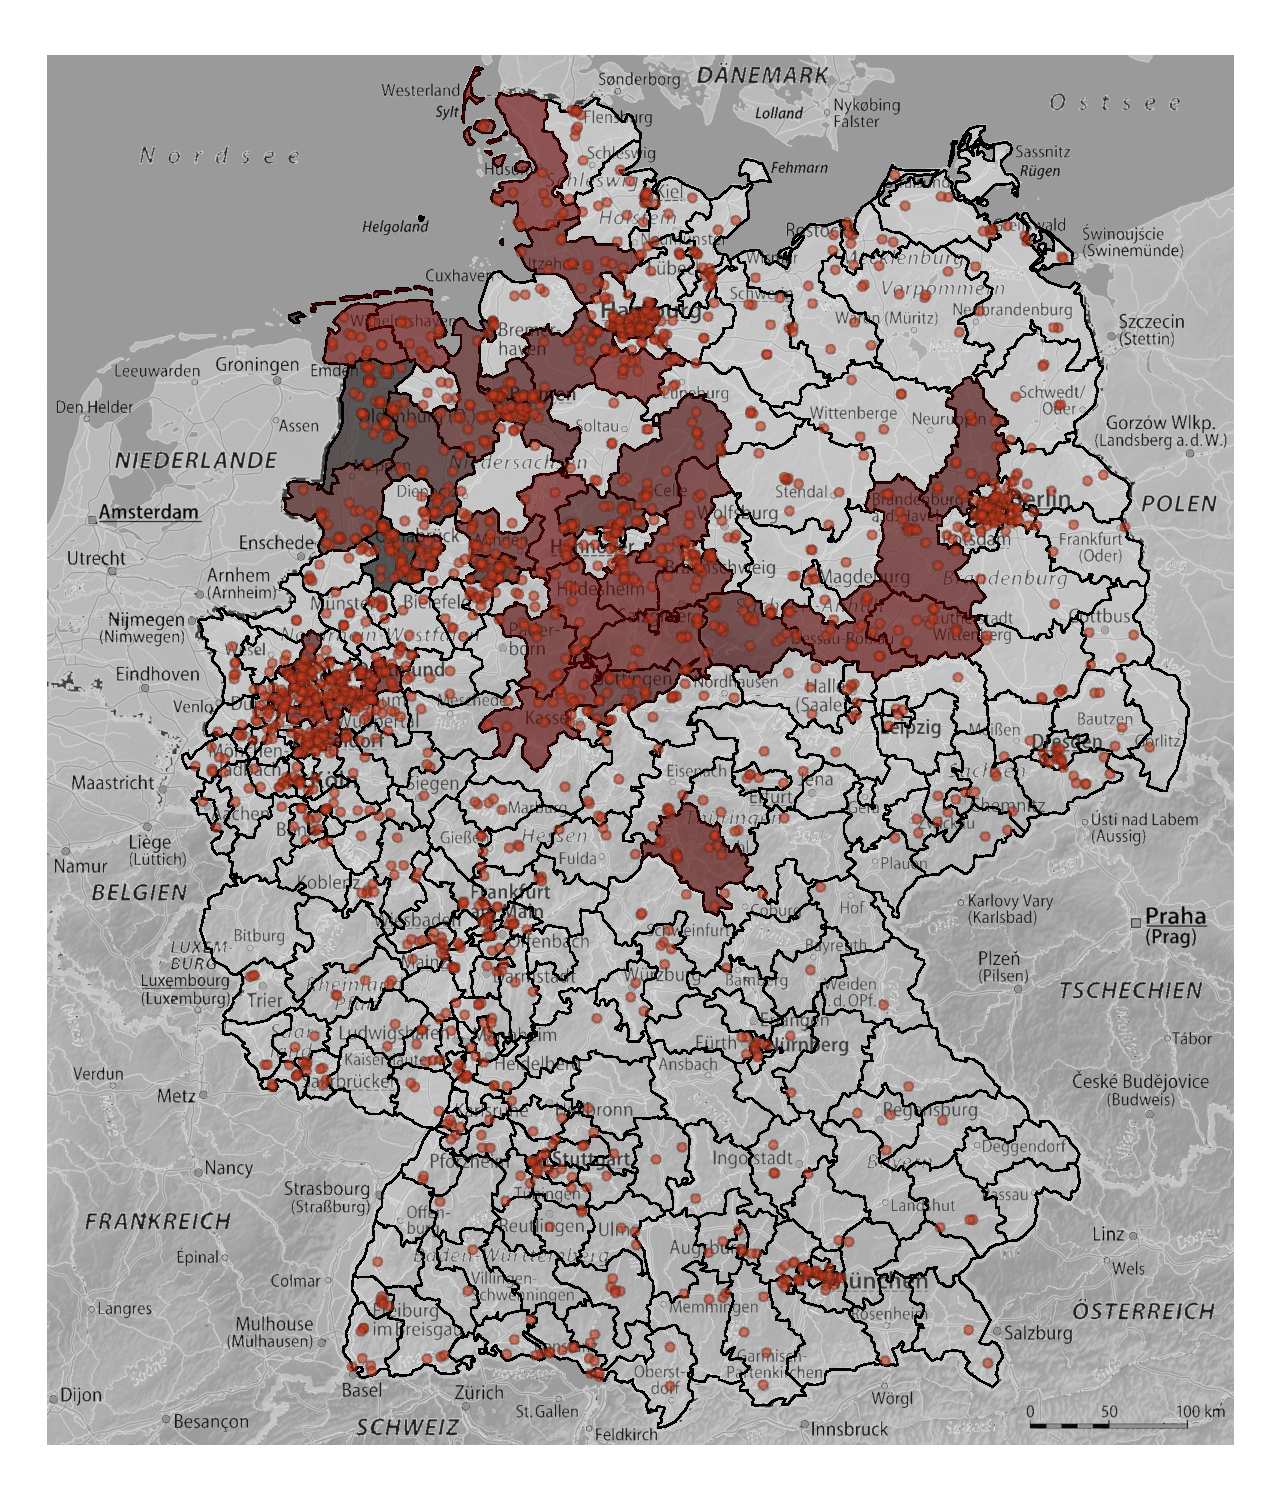
\includegraphics{fig/name_distribution.pdf}

\#\#\ldots{}

\ldots{}

\end{frame}

\section{Conclusion}\label{conclusion}

\begin{frame}{Conclusion}

\begin{itemize}
\tightlist
\item
  applications are diverse and many fold
\item
  the web is everywhere
\item
  web data formats are not only in the web (e.g.~EPub, Docx, KML are
  XML)
\item
  data extraction skills (e.g.~RegEx) are swiss army knives
\end{itemize}

\end{frame}

\end{document}
